The N-Queens puzzle is the problem of placing N chess queens on an NxN
chessboard so that no pair of two queens attack each
other~\cite{8queens}. The challenge of finding all the
distinct solutions to this problem is a good benchmark in designing
parallel algorithms.

The CLM solution considers the chess board as a graph where nodes exchange valid
configurations between each other. First, we start with the empty
state in the first row of the chess board. Then, each square adds its own
position to the state and sends the state down, to the next row. Once a square
receives new configurations, it attempts to add its position to the
configurations. If valid, that configuration is then sent, recursively, to the
next row, until all rows are traversed. At the end of the program, the nodes at
the bottom row will have all the valid configurations.

Since computation goes from the top row to the bottom row, not all placements of
nodes on threads may be equally performant. This is especially true because the
bottom rows tend to perform the most work. The best placement is then to split the
board vertically, so that, in optimal conditions, each thread gets the same
number of columns. Our experiments show that, on shared memory, it does not
matter much if we start with a bad placement since node stealing overcomes those
issues by improving load balancing dynamically. However, we noticed interesting
cache effects when prioritizing nodes in bottom rows. The N Queens program
builds and shares lists representing valid board states and needs to iterate
over those lists often when checking if a new position does not invalidate a state.
We thus used coordination axioms \texttt{set-default-priority(A, X)} and \texttt{set-cpu(A,
vertical(X, Y))}, where \texttt{X} is the row number (0 is the top row) and
\texttt{Y} is the column number.

Experimental results are presented in Fig.~\ref{results:nqueens}.
We first ran the coordinated program using dynamic partitioning (with work
stealing) and saw some performance improvements (\textbf{Coordinated}). However, using dynamic
partitioning is bad for memory locality since threads will steal nodes often.
We then added \texttt{set-static(A)} as a coordination axiom and saw
performance improvement (\textbf{Static}), especially when the board columns are perfectly
partitioned by the number of threads (in our case 13 threads).

\begin{topfig}
   \begin{center}
      \subfloat[]{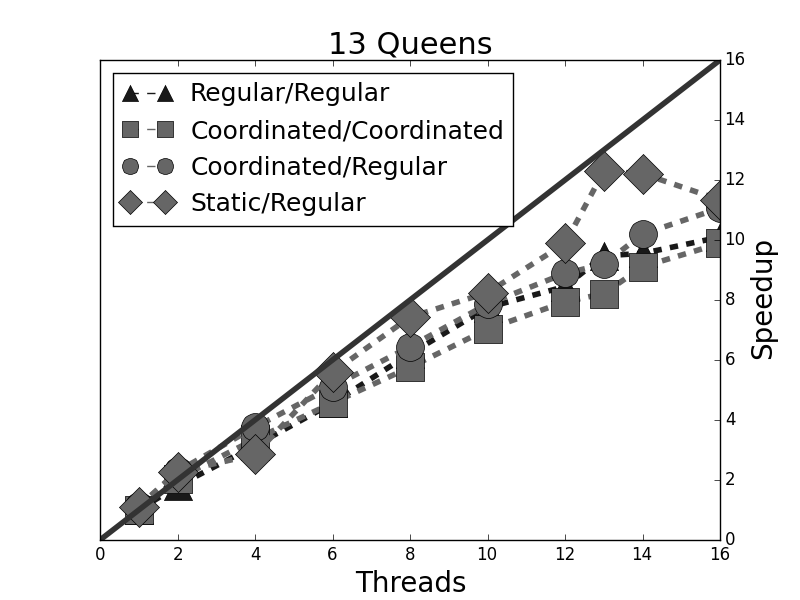
\includegraphics[width=5.5cm]{results/8queens-13.png}}
   \end{center}
   \scap{results:nqueens}{Experimental results for the 13 Queens program.
   Coordination works best when 1 column is assigned to one thread and bottom
   rows have higher priority.}
\end{topfig}
